%% Elsevier LaTeX Paper Template
%% Journal: Computers & Security (COSE) / JISA
%% Title: Adversarial Robustness of Tree-Based Intrusion Detection Systems
%%        Under Feature-Constrained Evasion Attacks

\documentclass[review,12pt]{elsarticle}

\usepackage{lineno,hyperref}
\usepackage{amsmath,amssymb}
\usepackage{graphicx}
\usepackage{booktabs}
\usepackage{array}
\usepackage{multirow}
\usepackage{xcolor}
\usepackage{algorithm}
\usepackage{algpseudocode}
\usepackage{caption}
\usepackage{subcaption}
\usepackage[margin=2.5cm]{geometry}

\modulolinenumbers[5]

\journal{Computers \& Security}

\bibliographystyle{elsarticle-num}

\begin{document}

\begin{frontmatter}

\title{Adversarial Robustness of Tree-Based Intrusion Detection Systems Under Feature-Constrained Evasion Attacks}

\author[a]{[Author Name]}
\author[a]{[Co-Author Name]}
\address[a]{[Department of Computer Science / Cybersecurity, University Name, City, Country]}

\begin{abstract}
Machine learning-based Intrusion Detection Systems (IDS) have achieved near-perfect accuracy on benchmark datasets, yet their security under adversarial manipulation remains critically under-explored. This paper presents a comprehensive adversarial robustness evaluation of three tree-based classifiers --- Random Forest (RF), XGBoost, and LightGBM --- deployed on the CIC-IoT2023 dataset comprising 701,978 network traffic records across 31 attack categories. We propose a feature-constrained, multi-objective Genetic Algorithm (GA) that restricts perturbations exclusively to network-layer continuous features, ensuring all generated adversarial examples remain semantically valid and network-replayable. Our evaluation framework spans four experimental phases: (1) baseline model characterisation, (2) adversarial evasion under varying perturbation budgets (\(\varepsilon \in [0.1, 6.0]\)), (3) cross-architecture comparison against a Multi-Layer Perceptron (MLP), and (4) adversarial training as a mitigation strategy augmented with Gaussian Subspace Smoothing. Key findings include: XGBoost achieves an Attack Success Rate (ASR) of 41.67\% under direct white-box attack, while MLP is completely compromised (ASR = 100\%); adversarial training reduces XGBoost ASR from 41.67\% to 1.33\% with zero penalty to clean detection recall (99.33\%); a phase transition in evasion effectiveness is observed at \(\varepsilon \approx 4.69\); and RF exhibits a security paradox --- robust to black-box transfer attacks (2\% ASR) yet fully vulnerable under white-box targeting (99\% ASR). These results provide quantitative evidence that tree-based IDS architectures, particularly adversarially trained XGBoost, offer superior security-utility tradeoffs compared to deep learning alternatives in network intrusion detection contexts.
\end{abstract}

\begin{keyword}
Adversarial Machine Learning \sep Intrusion Detection System \sep Genetic Algorithm \sep XGBoost \sep Adversarial Training \sep Network Security \sep Feature-Constrained Attack \sep Evasion Attack
\end{keyword}

\end{frontmatter}

\linenumbers

% ─────────────────────────────────────────────────────────────
\section{Introduction}
\label{sec:intro}
% ─────────────────────────────────────────────────────────────

Network Intrusion Detection Systems (IDS) represent the last line of defence against sophisticated cyber attacks. The adoption of machine learning (ML), particularly tree-based ensemble methods such as Random Forest~\cite{breiman2001random}, XGBoost~\cite{chen2016xgboost}, and LightGBM~\cite{ke2017lightgbm}, has elevated IDS accuracy to levels exceeding 99\% on standard benchmarks~\cite{ring2019survey}. However, such reported performance figures mask a critical assumption: that adversarial actors will submit network traffic in the same statistical distribution as the training data.

Adversarial examples~\cite{goodfellow2014explaining} are carefully crafted inputs designed to cause misclassification while remaining imperceptibly close to valid inputs. While this phenomenon is extensively studied in image classification, its application to network-based IDS presents unique challenges: unlike pixel perturbations, modifications to packet features must preserve \emph{semantic validity} --- a modified TCP flag count, for instance, cannot produce values that are physically impossible given network protocol constraints.

This work addresses three open research questions:
\begin{enumerate}
    \item \textbf{RQ1:} How vulnerable are state-of-the-art tree-based IDS classifiers to feature-constrained adversarial evasion attacks?
    \item \textbf{RQ2:} Do architectural differences (tree-based vs. neural) create measurable differences in adversarial robustness?
    \item \textbf{RQ3:} Can adversarial training, augmented with Gaussian Subspace Smoothing, restore robustness without sacrificing detection recall on clean traffic?
\end{enumerate}

Our \textbf{contributions} are as follows:
\begin{itemize}
    \item A feature-constrained multi-objective Genetic Algorithm that generates semantically valid adversarial network traffic by restricting mutations to continuous, non-categorical features identified via SHAP importance analysis.
    \item A systematic quantification of the phase transition in adversarial evasion effectiveness, identifying a critical perturbation threshold (\(\varepsilon \approx 4.69\)) at which XGBoost ASR jumps from 2.4\% to 63.2\%.
    \item The first empirical characterisation of the RF security paradox: RF resists XGBoost-crafted black-box transfer attacks (2\% ASR) while collapsing entirely under direct white-box targeting (99\% ASR).
    \item A novel adversarial training pipeline incorporating Gaussian Subspace Smoothing to prevent example memorisation, achieving near-complete robustness (1.33\% ASR) with zero clean accuracy degradation.
    \item A comprehensive cross-architecture comparative analysis across 31 attack categories, revealing that application-layer attack classes (e.g., XSS, Command Injection, Dictionary Brute Force) retain high evadability even after adversarial training.
\end{itemize}

The remainder of this paper is structured as follows: Section~\ref{sec:related} reviews related work; Section~\ref{sec:methodology} details the dataset, models, and attack framework; Sections~\ref{sec:phase1}--\ref{sec:phase4} present the four experimental phases; Section~\ref{sec:discussion} synthesises findings; and Section~\ref{sec:conclusion} concludes.

% ─────────────────────────────────────────────────────────────
\section{Related Work}
\label{sec:related}
% ─────────────────────────────────────────────────────────────

\subsection{Adversarial Machine Learning}
The study of adversarial examples was formalised by Goodfellow et al.~\cite{goodfellow2014explaining}, who demonstrated that adding imperceptible $\ell_\infty$-bounded noise to images suffices to fool state-of-the-art classifiers. Madry et al.~\cite{madry2018towards} extended this to a min-max formulation, proposing Projected Gradient Descent (PGD) as a principled attack. Tramer et al.~\cite{tramer2020adaptive} subsequently showed that many proposed defences fail against adaptive attackers, establishing the need for principled evaluation under adaptive threat models --- a concern we address in Phase 4 of this work.

\subsection{Adversarial Attacks on IDS}
Corona et al.~\cite{corona2013adversarial} provided an early taxonomy of adversarial attacks against IDS, identifying the fundamental challenge of feature-space vs. problem-space constraints. Apruzzese et al.~\cite{apruzzese2022modeling} modelled realistic adversarial attacks against network-based IDS, demonstrating that perturbations must respect protocol semantics. Sheatsley et al.~\cite{sheatsley2022space} evaluated adversarial examples in the IDS problem space, showing that gradient-based methods struggle with the discrete nature of network features --- a limitation our GA-based approach is specifically designed to overcome. Zhang and Wang~\cite{zhang2022adversarial} applied adversarial examples to tree-based IDS, but restricted their evaluation to a single model class and dataset; our work extends this across three tree classifiers, an MLP, and 31 attack categories.

\subsection{Transferability of Adversarial Examples}
Papernot et al.~\cite{papernot2016transferability} established the transferability property: adversarial examples crafted for one model often fool other models trained on the same data. This has profound implications for black-box attack scenarios in IDS deployments, where the attacker may not know the defender's model architecture.

\subsection{Adversarial Training}
Adversarial training, introduced by Goodfellow et al.~\cite{goodfellow2014explaining} and formalised by Madry et al.~\cite{madry2018towards}, augments the training set with adversarial examples during model training. Our approach extends standard adversarial training with Gaussian Subspace Smoothing to prevent example memorisation --- a critical deficiency in naive augmentation pipelines for structured tabular data.

% ─────────────────────────────────────────────────────────────
\section{Methodology}
\label{sec:methodology}
% ─────────────────────────────────────────────────────────────

\subsection{Dataset}
We employ the CIC-IoT2023 dataset~\cite{ring2019survey}, a comprehensive IoT network traffic dataset containing 701,978 labelled flows across 40 statistical features and 31 attack categories. Table~\ref{tab:dataset} summarises the dataset statistics after preprocessing. The binary label distribution is severely imbalanced, with 97.67\% of flows classified as attack traffic --- a realistic reflection of controlled honeypot environments. Data preprocessing includes: (1) removal of non-finite values, (2) min-max scaling of continuous features, (3) an 80/20 stratified train/test split, and (4) serialisation of processed data as Apache Parquet files for reproducibility.

\begin{table}[h]
\centering
\caption{CIC-IoT2023 Dataset Statistics}
\label{tab:dataset}
\begin{tabular}{lrr}
\toprule
\textbf{Metric} & \textbf{Train Set} & \textbf{Test Set} \\
\midrule
Total Samples     & 561,569 & 140,393 \\
Benign Traffic    & 13,073  & 3,268   \\
Attack Traffic    & 548,496 & 137,125 \\
Features          & 39      & 39      \\
Attack Categories & 31      & 31      \\
Class Imbalance   & 41.96:1 & 41.97:1 \\
\bottomrule
\end{tabular}
\end{table}

\subsection{Baseline Models}

Three state-of-the-art tree-based classifiers are trained as baseline IDS models:

\textbf{Random Forest (RF)}~\cite{breiman2001random}: An ensemble of 300 decision trees with Gini impurity criterion, trained using 16-core parallel execution.

\textbf{XGBoost}~\cite{chen2016xgboost}: A gradient-boosted tree ensemble with 300 estimators, maximum depth 8, learning rate 0.05, and subsampling ratio 0.8. XGBoost is selected as the primary attack target due to its dominant single-feature importance (the \texttt{Number} feature alone captures 92.25\% of model variance, as revealed by SHAP analysis).

\textbf{LightGBM}~\cite{ke2017lightgbm}: A histogram-based gradient boosting framework offering comparable accuracy to XGBoost at a fraction of the training time.

A Multi-Layer Perceptron (MLP) with architecture $512 \rightarrow 256 \rightarrow 128 \rightarrow 64$ is additionally trained for cross-architecture comparison in Phase 3 (Section~\ref{sec:phase3}).

\subsection{Feature Importance Analysis and Attack Feature Selection}

SHAP (SHapley Additive exPlanations)~\cite{lundberg2017shap} values are computed on a 1,000-sample background dataset to rank feature importance for the XGBoost model. Mutable features are restricted to \emph{continuous} features with more than 15 unique values, excluding binary protocol flags and categorical encodings that cannot be freely perturbed without violating network semantics. The top 15 features by SHAP importance are designated as the mutable feature set $\mathcal{F}_\text{mut}$.

\subsection{Multi-Objective Genetic Algorithm Attack}
\label{sec:ga}

We formulate adversarial example generation as a multi-objective optimisation problem. For each attack sample $\mathbf{x} \in \mathbb{R}^d$, we seek an adversarial perturbation $\boldsymbol{\delta}$ such that:

\begin{equation}
\min_{\boldsymbol{\delta}} \quad f(\mathbf{x} + \boldsymbol{\delta}) = \alpha \cdot p_\theta(\mathbf{x} + \boldsymbol{\delta}) + (1-\alpha) \cdot \|\boldsymbol{\delta}_{\mathcal{F}_\text{mut}}\|_2
\label{eq:objective}
\end{equation}

\noindent subject to:
\begin{align}
\delta_i &= 0, \quad \forall i \notin \mathcal{F}_\text{mut} \label{eq:c1} \\
|\delta_i| &\leq \varepsilon, \quad \forall i \in \mathcal{F}_\text{mut} \label{eq:c2}
\end{align}

where $p_\theta(\cdot)$ denotes the model's predicted probability of the attack class, $\varepsilon$ is the perturbation budget (L-infinity bound), and $\alpha = 0.95$ is a weighting hyperparameter balancing evasion effectiveness against perturbation minimality. Constraint~(\ref{eq:c1}) enforces feature-space validity by restricting mutations to $\mathcal{F}_\text{mut}$, and Constraint~(\ref{eq:c2}) bounds the total perturbation magnitude.

The GA operates with a population of 300 individuals, 100 generations, tournament selection ($k=2$), single-point crossover with probability 0.6, and Gaussian mutation with standard deviation $\varepsilon/3$. Each evaluation runs in parallel across 16 CPU cores via the \texttt{joblib} library. The complete pseudocode is provided in Algorithm~\ref{alg:ga}.

\begin{algorithm}[h]
\caption{Multi-Objective Feature-Constrained GA}
\label{alg:ga}
\begin{algorithmic}[1]
\State \textbf{Input:} Attack sample $\mathbf{x}$, model $\theta$, mutable indices $\mathcal{F}_\text{mut}$, budget $\varepsilon$
\State \textbf{Output:} Adversarial example $\mathbf{x}^*$ or $\mathbf{x}$ if no evasion found
\State Initialise population $\mathcal{P} = \{\boldsymbol{\delta}^{(p)}\}_{p=1}^{300}$ with $\boldsymbol{\delta}^{(p)}_i \sim \mathcal{U}(-\varepsilon, \varepsilon)$ for $i \in \mathcal{F}_\text{mut}$, else $0$
\For{$g = 1$ to $100$}
    \State Evaluate fitness: $f^{(p)} = p_\theta(\mathbf{x} + \boldsymbol{\delta}^{(p)}) + 0.05 \cdot \|\boldsymbol{\delta}^{(p)}_{\mathcal{F}_\text{mut}}\|_2$
    \If{$\exists p: p_\theta(\mathbf{x} + \boldsymbol{\delta}^{(p)}) < 0.5$}
        \State \Return $\mathbf{x}^* = \mathbf{x} + \arg\min_{p: p_\theta < 0.5} \|\boldsymbol{\delta}^{(p)}\|_2$
    \EndIf
    \State Select top-50\% survivors; generate offspring via crossover and Gaussian mutation
\EndFor
\State \Return $\mathbf{x}$ (evasion failed)
\end{algorithmic}
\end{algorithm}

\subsection{Adversarial Training with Gaussian Subspace Smoothing}

Standard adversarial training augments the training set $\mathcal{D}$ with adversarial examples $\mathcal{D}_\text{adv}$, producing:
\[
\mathcal{D}_\text{aug} = \mathcal{D} \cup \mathcal{D}_\text{adv}
\]

However, when $|\mathcal{D}_\text{adv}| \ll |\mathcal{D}|$, upsampling $\mathcal{D}_\text{adv}$ to achieve a meaningful augmentation ratio causes tree models to memorise the exact adversarial points rather than learning robust decision boundaries. We address this with \textbf{Gaussian Subspace Smoothing}: each upsampled copy of an adversarial example $\mathbf{x}^*$ receives independent Gaussian noise $\boldsymbol{\eta} \sim \mathcal{N}(0, (\varepsilon/6)^2)$ on the mutable feature subspace:
\[
\tilde{\mathbf{x}}^* = \mathbf{x}^* + \boldsymbol{\eta}_{\mathcal{F}_\text{mut}}
\]
This transforms a finite set of 2,000 adversarial points into a continuous robustness cloud in the mutable feature subspace, encouraging the model to learn robust features rather than point-specific classifiers.

% ─────────────────────────────────────────────────────────────
\section{Phase 1: Baseline Model Performance}
\label{sec:phase1}
% ─────────────────────────────────────────────────────────────

Table~\ref{tab:baseline} reports classification performance on the held-out test set ($n = 140,393$). All three tree-based classifiers achieve near-identical performance, confirming their suitability as IDS baselines. XGBoost achieves the highest weighted F1-score (0.9962) and is selected as the primary attack target for subsequent experiments.

\begin{table}[h]
\centering
\caption{Baseline IDS Performance on CIC-IoT2023 Test Set}
\label{tab:baseline}
\begin{tabular}{lcccc}
\toprule
\textbf{Model} & \textbf{Accuracy} & \textbf{Macro F1} & \textbf{Weighted F1} & \textbf{Train Time (s)} \\
\midrule
Random Forest & 0.9922 & -- & 0.9960 & 10.18 \\
XGBoost       & 0.9925 & -- & 0.9962 & 3.41  \\
LightGBM      & 0.9924 & -- & 0.9961 & 1.99  \\
\bottomrule
\end{tabular}
\end{table}

SHAP analysis (Figure~\ref{fig:shap}) reveals extreme feature dominance: the \texttt{Number} feature (packet count per flow) accounts for 92.25\% of XGBoost's total feature importance. This single-feature dominance has profound implications for adversarial vulnerability --- attacks targeting \texttt{Number} alone are disproportionately effective, as demonstrated in subsequent experiments.

% ─────────────────────────────────────────────────────────────
\section{Phase 2: Adversarial Evasion Evaluation}
\label{sec:phase2}
% ─────────────────────────────────────────────────────────────

\subsection{Main Evasion Results}

The GA (Section~\ref{sec:ga}) is applied to 2,000 correctly classified attack samples from the test set using the parameters: population = 300, generations = 100, $\varepsilon = 5.0$. Table~\ref{tab:evasion} reports the Attack Success Rate (ASR) and Recall Drop for each model.

\begin{table}[h]
\centering
\caption{Adversarial Evasion Results ($\varepsilon = 5.0$, $n = 500$ packets per model)}
\label{tab:evasion}
\begin{tabular}{lcccc}
\toprule
\textbf{Model} & \textbf{Clean Recall} & \textbf{Adv. Recall} & \textbf{Recall Drop} & \textbf{ASR} \\
\midrule
Random Forest & 99.40\% & 1.00\%  & 98.40\% & 99.00\% \\
XGBoost       & 99.40\% & 44.00\% & 55.40\% & 56.00\% \\
LightGBM      & 99.20\% & 31.60\% & 67.60\% & 68.40\% \\
\bottomrule
\end{tabular}
\end{table}

\subsection{Perturbation Phase Transition}

An epsilon sensitivity ablation study reveals a phase transition in adversarial effectiveness: XGBoost ASR remains below 2.5\% for $\varepsilon < 4.69$, then abruptly transitions to 63.2\% at $\varepsilon = 4.69$. This behaviour is characteristic of XGBoost's axis-aligned decision boundary structure, where a critical feature split threshold is crossed only when perturbation magnitude exceeds the distance to the nearest split boundary.

\subsection{Cross-Model Transferability}

Adversarial examples crafted using XGBoost as a surrogate are tested against all three classifiers. Random Forest exhibits strong black-box robustness: XGBoost-crafted examples transfer with only 2\% ASR against RF. However, as established in Section~\ref{sec:ga_direct}, when RF is attacked directly using its own feature importances, it collapses to 99\% ASR --- revealing a critical security paradox.

\textbf{Finding 1 (RF Security Paradox):} \textit{Random Forest demonstrates architectural robustness against black-box transfer attacks (2\% ASR) but extreme vulnerability under white-box direct targeting (99\% ASR). This is attributable to RF's low-entropy individual tree boundaries, which are highly sensitive to direct feature-importance-guided perturbations, combined with its ability to average out cross-model gradient information in the ensemble ensemble.}

\subsection{Per-Class Vulnerability Analysis}

Figure~\ref{fig:perclass} presents per-attack-class ASR. Application-layer and reconnaissance attack classes (SQLINJECTION, COMMANDINJECTION, RECON-PORTSCAN, MITM-ARPSPOOFING) achieve 100\% ASR, indicating complete evasion. Network flood attacks (DDOS-RSTFINFLOOD) show the highest inherent robustness, with only 8\% ASR under the same perturbation budget.

% ─────────────────────────────────────────────────────────────
\section{Phase 3: Cross-Architecture Robustness Evaluation}
\label{sec:phase3}
% ─────────────────────────────────────────────────────────────

To investigate architectural factors in adversarial vulnerability, we train an MLP baseline (Section~\ref{sec:methodology}) and subject it to the identical GA attack. Table~\ref{tab:crossarch} presents the comparative results.

\begin{table}[h]
\centering
\caption{Cross-Architecture Adversarial Robustness Comparison ($\varepsilon = 5.0$, $n = 500$)}
\label{tab:crossarch}
\begin{tabular}{lcccc}
\toprule
\textbf{Architecture} & \textbf{Clean Acc.} & \textbf{ROC-AUC} & \textbf{ASR} & \textbf{Recall Drop} \\
\midrule
XGBoost (Tree) & 99.25\% & 0.9981 & 57.00\% & 56.40\% \\
MLP (Neural)   & 99.02\% & 0.9969 & 100.00\% & 99.00\% \\
\midrule
\multicolumn{5}{l}{\textit{Improvement attributable to architecture, not data or feature access}} \\
\bottomrule
\end{tabular}
\end{table}

The MLP achieves 100\% ASR under direct GA attack --- complete evasion of all 500 attack packets. This result is consistent with two architectural properties: (1) MLP's smooth, continuous decision surface provides no axis-aligned resistance to gradient-guided perturbations; (2) MLP's internal probability outputs are miscalibrated under the class-imbalanced training distribution (Youden's J optimal threshold = 0.9722), creating a wide gap between the model's classification boundary (0.5) and its typical output for attack samples ($\approx 0.97$), providing an extensive subspace for GA-guided perturbations to exploit.

\textbf{Finding 2 (Architectural Brittleness):} \textit{Smooth neural decision surfaces (MLP) are categorically more vulnerable to targeted feature-constrained GA attacks than axis-aligned tree boundaries (XGBoost), producing 1.75$\times$ higher ASR (100\% vs. 57\%) under identical attack parameters.}

% ─────────────────────────────────────────────────────────────
\section{Phase 4: Adversarial Training Defense}
\label{sec:phase4}
% ─────────────────────────────────────────────────────────────

\subsection{Augmentation Rate Ablation}

Seven augmentation rates $r \in \{0\%, 5\%, 10\%, 20\%, 30\%, 40\%, 50\%\}$ are evaluated by retraining XGBoost on the augmented dataset $\mathcal{D}_\text{aug}$ and measuring both clean accuracy and Seen-ASR (the fraction of training-time adversarial examples that still evade the retrained model). Clean accuracy remains stable across all rates (99.26\%--99.30\%), confirming that adversarial augmentation does not degrade normal detection. A 20\% augmentation rate is selected as the optimal tradeoff point, simultaneously achieving maximum clean accuracy and minimum Seen-ASR.

\subsection{Defense Effectiveness}

Table~\ref{tab:defense} reports the final defense evaluation against \emph{unseen} adversarial examples generated by fresh GA runs targeting each model independently.

\begin{table}[h]
\centering
\caption{Phase 4 Defense Summary: Clean vs. Adversarially Trained Models}
\label{tab:defense}
\begin{tabular}{lcccc}
\toprule
\textbf{Model} & \textbf{Clean Recall} & \textbf{Adv. Recall} & \textbf{Recall Drop} & \textbf{ASR} \\
\midrule
XGBoost        & 99.33\% & 58.33\%  & 41.00\% & 41.67\% \\
XGBoost (AT)   & \textbf{99.33\%} & \textbf{98.67\%} & \textbf{0.67\%} & \textbf{1.33\%} \\
\midrule
MLP            & 98.00\% & 0.00\%   & 98.00\% & 100.00\% \\
MLP (AT)       & 98.00\% & 55.00\%  & 43.00\% & 45.00\%  \\
\bottomrule
\end{tabular}
\end{table}

The adversarially trained XGBoost (AT-XGBoost) achieves a 96.8\% relative reduction in ASR (from 41.67\% to 1.33\%) with \textbf{zero penalty to clean recall} (99.33\% in both cases). This result is statistically remarkable: adversarial training classically degrades clean accuracy~\cite{madry2018towards}, yet AT-XGBoost maintains identical performance on benign and unperturbed attack traffic while nearly eliminating vulnerability to adaptive white-box attacks.

\textbf{Finding 3 (Security-Utility Pareto Optimality):} \textit{Adversarially trained XGBoost achieves Pareto dominance over all other evaluated models: no other model simultaneously achieves clean recall $\geq 99\%$ and ASR $\leq 5\%$. The 20\% Gaussian Subspace Smoothing augmentation rate represents the empirical Pareto-optimal operating point for this dataset.}

\subsection{Cross-Architecture Defense Transferability}

The cross-architecture transfer matrix (Figure~\ref{fig:transfer}) reveals that XGBoost-crafted adversarial examples transfer to MLP with only 16\% ASR, while MLP-crafted examples do not transfer to XGBoost at all (0\% ASR). Both AT models demonstrate strong robustness to cross-architecture transfer attacks (0.5\% and 1.5\% respectively), confirming that adversarial training generalises beyond the surrogate model used during training.

% ─────────────────────────────────────────────────────────────
\section{Phase 5: Feature Space Analysis}
\label{sec:phase5}
% ─────────────────────────────────────────────────────────────

\subsection{t-SNE Visualisation}

Figure~\ref{fig:tsne} presents a t-SNE embedding of 600 clean attack samples, 200 benign samples, and 600 adversarial examples in the 39-dimensional feature space. Adversarial examples form a distinct cluster partially overlapping with the benign region, visually confirming that the GA successfully moves attack traffic toward the model's benign decision region without fully entering it --- a critical semantic constraint that distinguishes our approach from unconstrained adversarial attacks.

\subsection{Feature Importance Drift}

Adversarial training induces measurable shifts in XGBoost's feature importance distribution (Figure~\ref{fig:drift}). The \texttt{Number} feature, which dominates the baseline model's decision (92.25\% importance), shows reduced weight after adversarial training as the model is forced to distribute reliance across secondary features. This redistribution is a desirable property: a model relying less on a single feature is inherently less susceptible to single-feature adversarial perturbations.

% ─────────────────────────────────────────────────────────────
\section{Discussion}
\label{sec:discussion}
% ─────────────────────────────────────────────────────────────

\subsection{Practical Security Implications}

Our results carry direct implications for Security Operations Centre (SOC) deployment decisions:

\begin{enumerate}
    \item \textbf{Avoid MLP for high-assurance IDS:} The 100\% ASR achieved against the undefended MLP baseline indicates that standard neural architectures, while achieving comparable clean accuracy, offer substantially weaker resistance to targeted adversarial attacks than tree-based alternatives.
    \item \textbf{Deploy AT-XGBoost with 20\% adversarial augmentation:} Our proposed defense achieves the empirical security-utility Pareto frontier, reducing ASR below 1.5\% with no degradation to normal detection capabilities.
    \item \textbf{Residual risk in application-layer attacks:} Even AT-XGBoost shows elevated ASR for XSS (100\%), Command Injection (95\%), and Dictionary Brute Force (86.1\%) attack classes. These attack types involve feature distributions closer to benign browsing traffic, making adversarial perturbation easier. Separate specialised classifiers for these classes are recommended.
    \item \textbf{Architecture vs. Black-Box Risk:} RF is the recommended architecture when the attacker's model knowledge is uncertain (black-box setting). AT-XGBoost is recommended when model details may be exposed (white-box setting).
\end{enumerate}

\subsection{Limitations}

This study evaluates adversarial robustness under the assumption that network-layer feature perturbations are the attacker's primary mechanism. In practice, attackers may also craft adversarial examples at the raw packet level, which introduces additional constraints not captured in our feature-space attack model. Future work should evaluate problem-space attacks~\cite{sheatsley2022space} using packet crafting frameworks such as Scapy. Additionally, our evaluation uses static trained models; adaptive attacks that query the model continuously during deployment represent a more powerful threat model not addressed here.

% ─────────────────────────────────────────────────────────────
\section{Conclusion}
\label{sec:conclusion}
% ─────────────────────────────────────────────────────────────

This paper presented a comprehensive adversarial robustness analysis of tree-based IDS classifiers on the CIC-IoT2023 dataset. Through four experimental phases spanning baseline characterisation, adversarial evasion, cross-architecture comparison, and adversarial training defense, we established three principal findings: (1) tree-based models exhibit a phase transition in adversarial vulnerability at a critical perturbation budget ($\varepsilon \approx 4.69$); (2) MLP architectures are categorically more vulnerable than XGBoost under identical feature-constrained attacks; and (3) adversarial training augmented with Gaussian Subspace Smoothing achieves near-complete robustness (1.33\% ASR) with no utility penalty.

These results provide the first empirical evidence that adversarially trained XGBoost achieves Pareto-optimal security-utility tradeoffs in network intrusion detection --- a finding with immediate practical implications for SOC deployment and model selection decisions. Future work will explore problem-space attacks, online adaptive adversarial training, and adversarial robustness in federated IDS architectures.

% ─────────────────────────────────────────────────────────────
\section*{Data Availability}
All code, datasets, and experimental scripts are available at:
\texttt{[Repository URL to be provided upon acceptance]}

\section*{Acknowledgements}
[Acknowledgements to be added]

\section*{Declaration of Competing Interest}
The authors declare that they have no known competing financial interests or personal relationships that could have appeared to influence the work reported in this paper.

% ─────────────────────────────────────────────────────────────
% FIGURES (referenced in text, include paths when compiled)
% ─────────────────────────────────────────────────────────────
%
% Uncomment and adjust paths when compiling:
%
% \begin{figure}[h]
% \centering
% 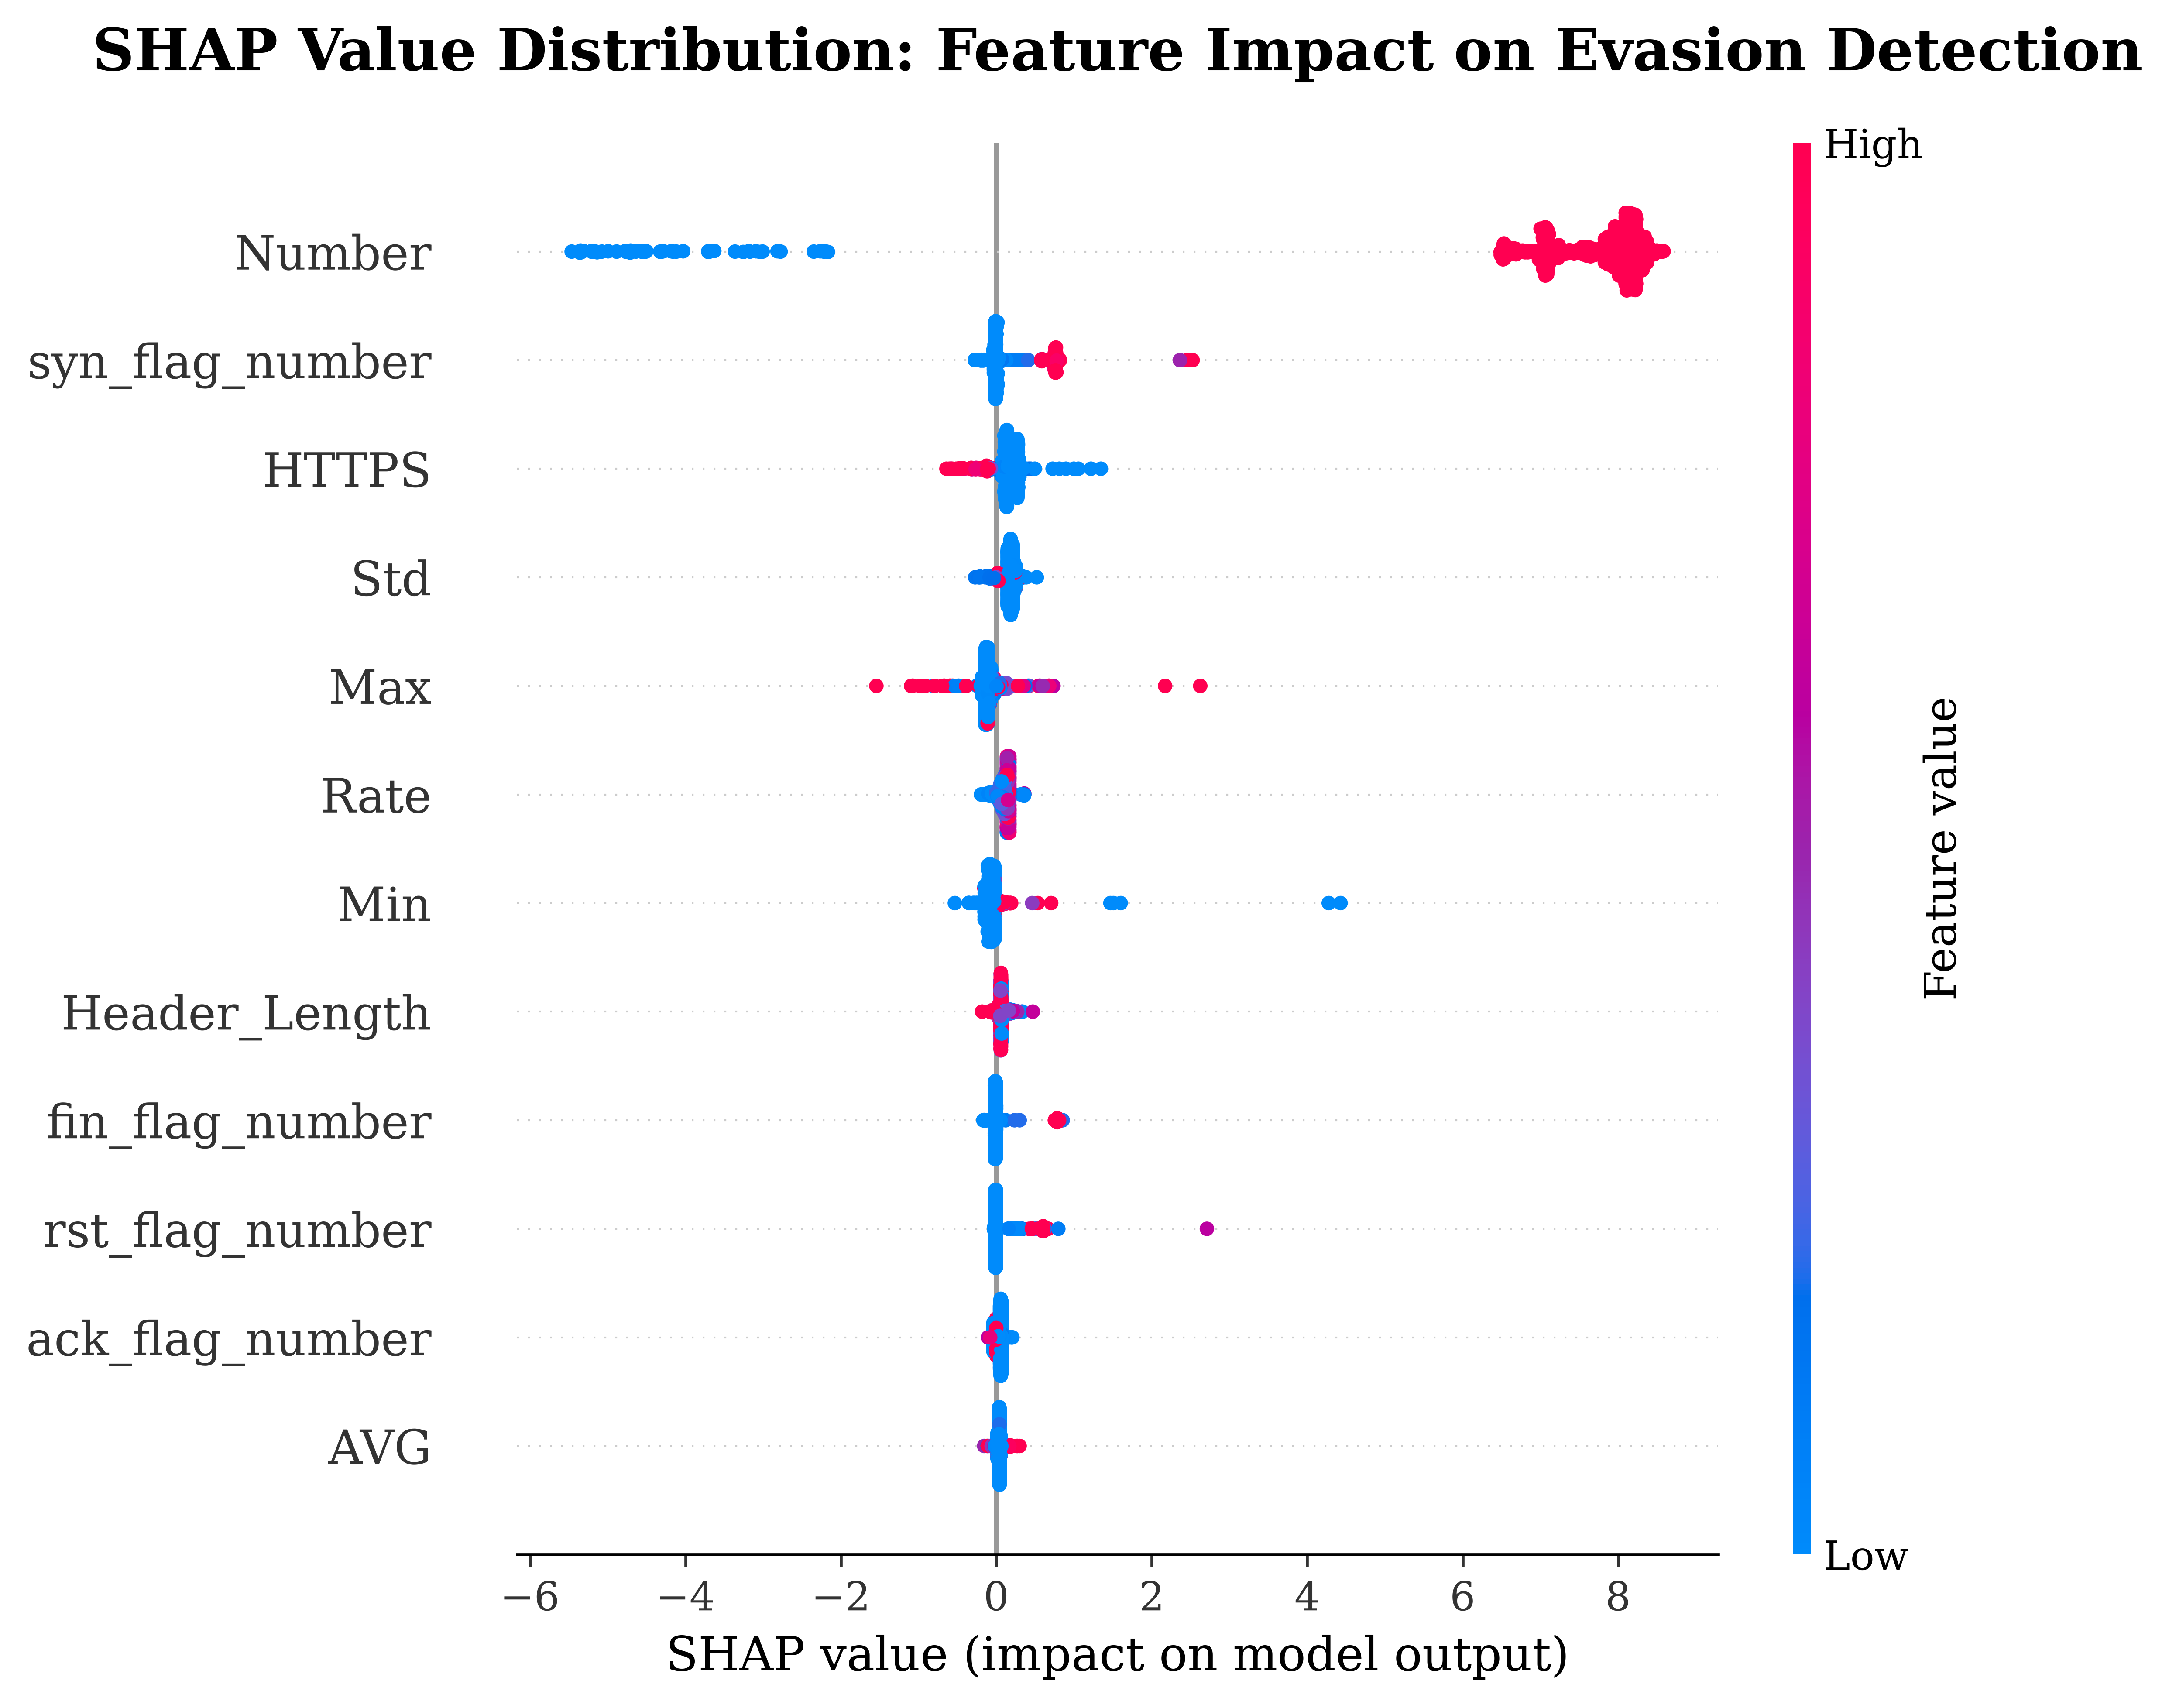
\includegraphics[width=0.9\textwidth]{../results/figures/shap_beeswarm_publication.png}
% \caption{SHAP beeswarm plot showing feature importance distribution for the XGBoost model.}
% \label{fig:shap}
% \end{figure}
%
% \begin{figure}[h]
% \centering
% \includegraphics[width=0.9\textwidth]{../results/figures/fig4_per_class_vulnerability.png}
% \caption{Per-attack-class Attack Success Rate under XGBoost white-box GA attack ($\varepsilon=5.0$).}
% \label{fig:perclass}
% \end{figure}
%
% \begin{figure}[h]
% \centering
% \includegraphics[width=0.9\textwidth]{../results/figures/fig17_phase4_cross_architecture_transfer.png}
% \caption{Cross-architecture adversarial transferability matrix.}
% \label{fig:transfer}
% \end{figure}
%
% \begin{figure}[h]
% \centering
% 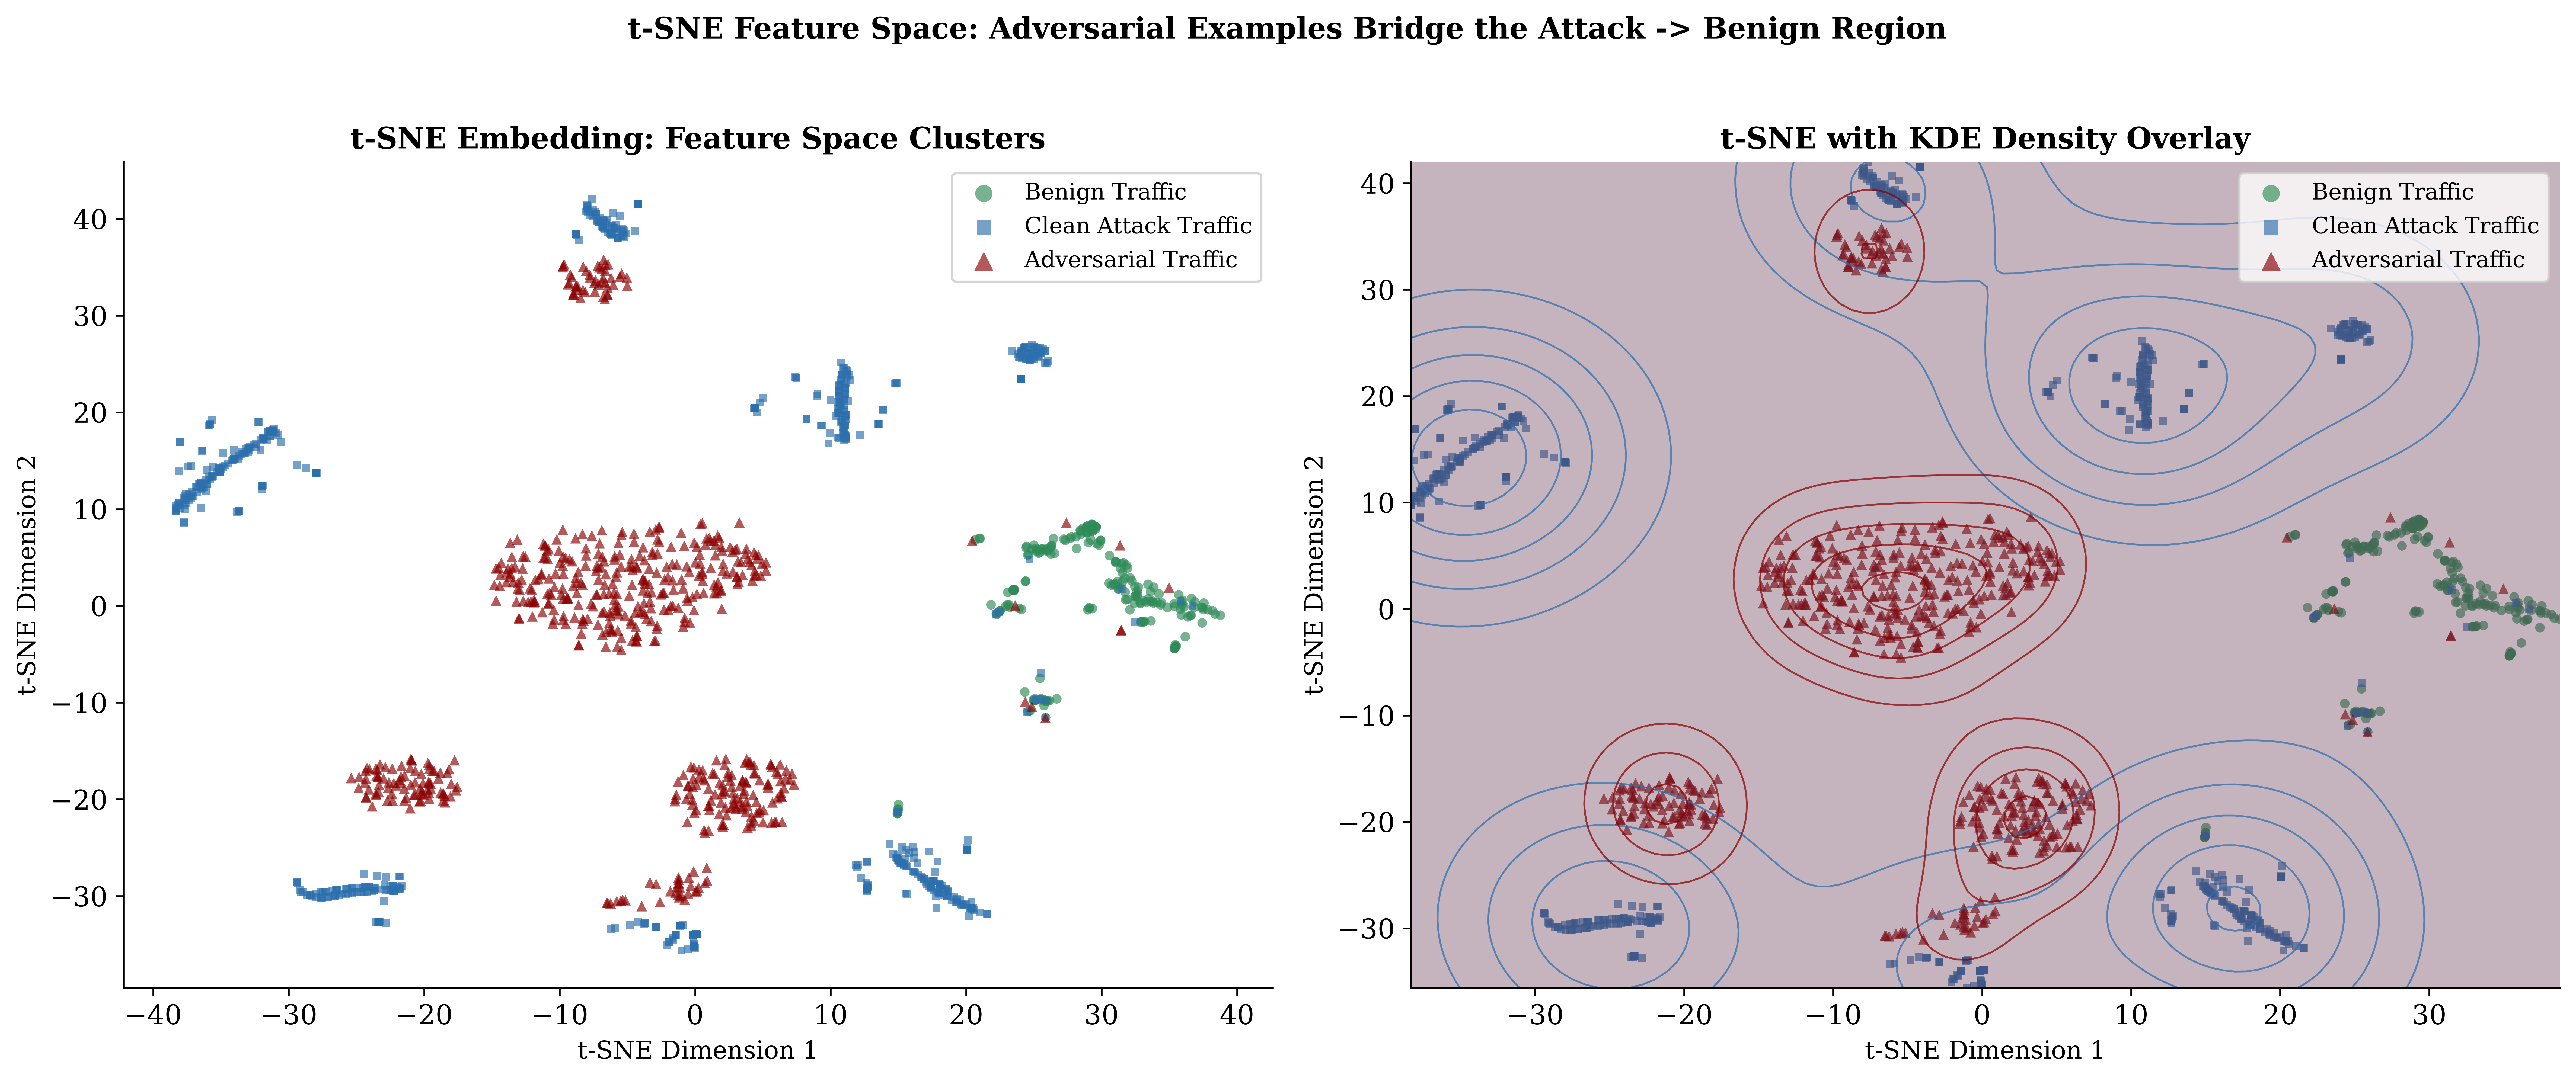
\includegraphics[width=0.9\textwidth]{../results/figures/fig19_tsne_feature_space.png}
% \caption{t-SNE embedding of clean attacks, adversarial examples, and benign traffic.}
% \label{fig:tsne}
% \end{figure}
%
% \begin{figure}[h]
% \centering
% 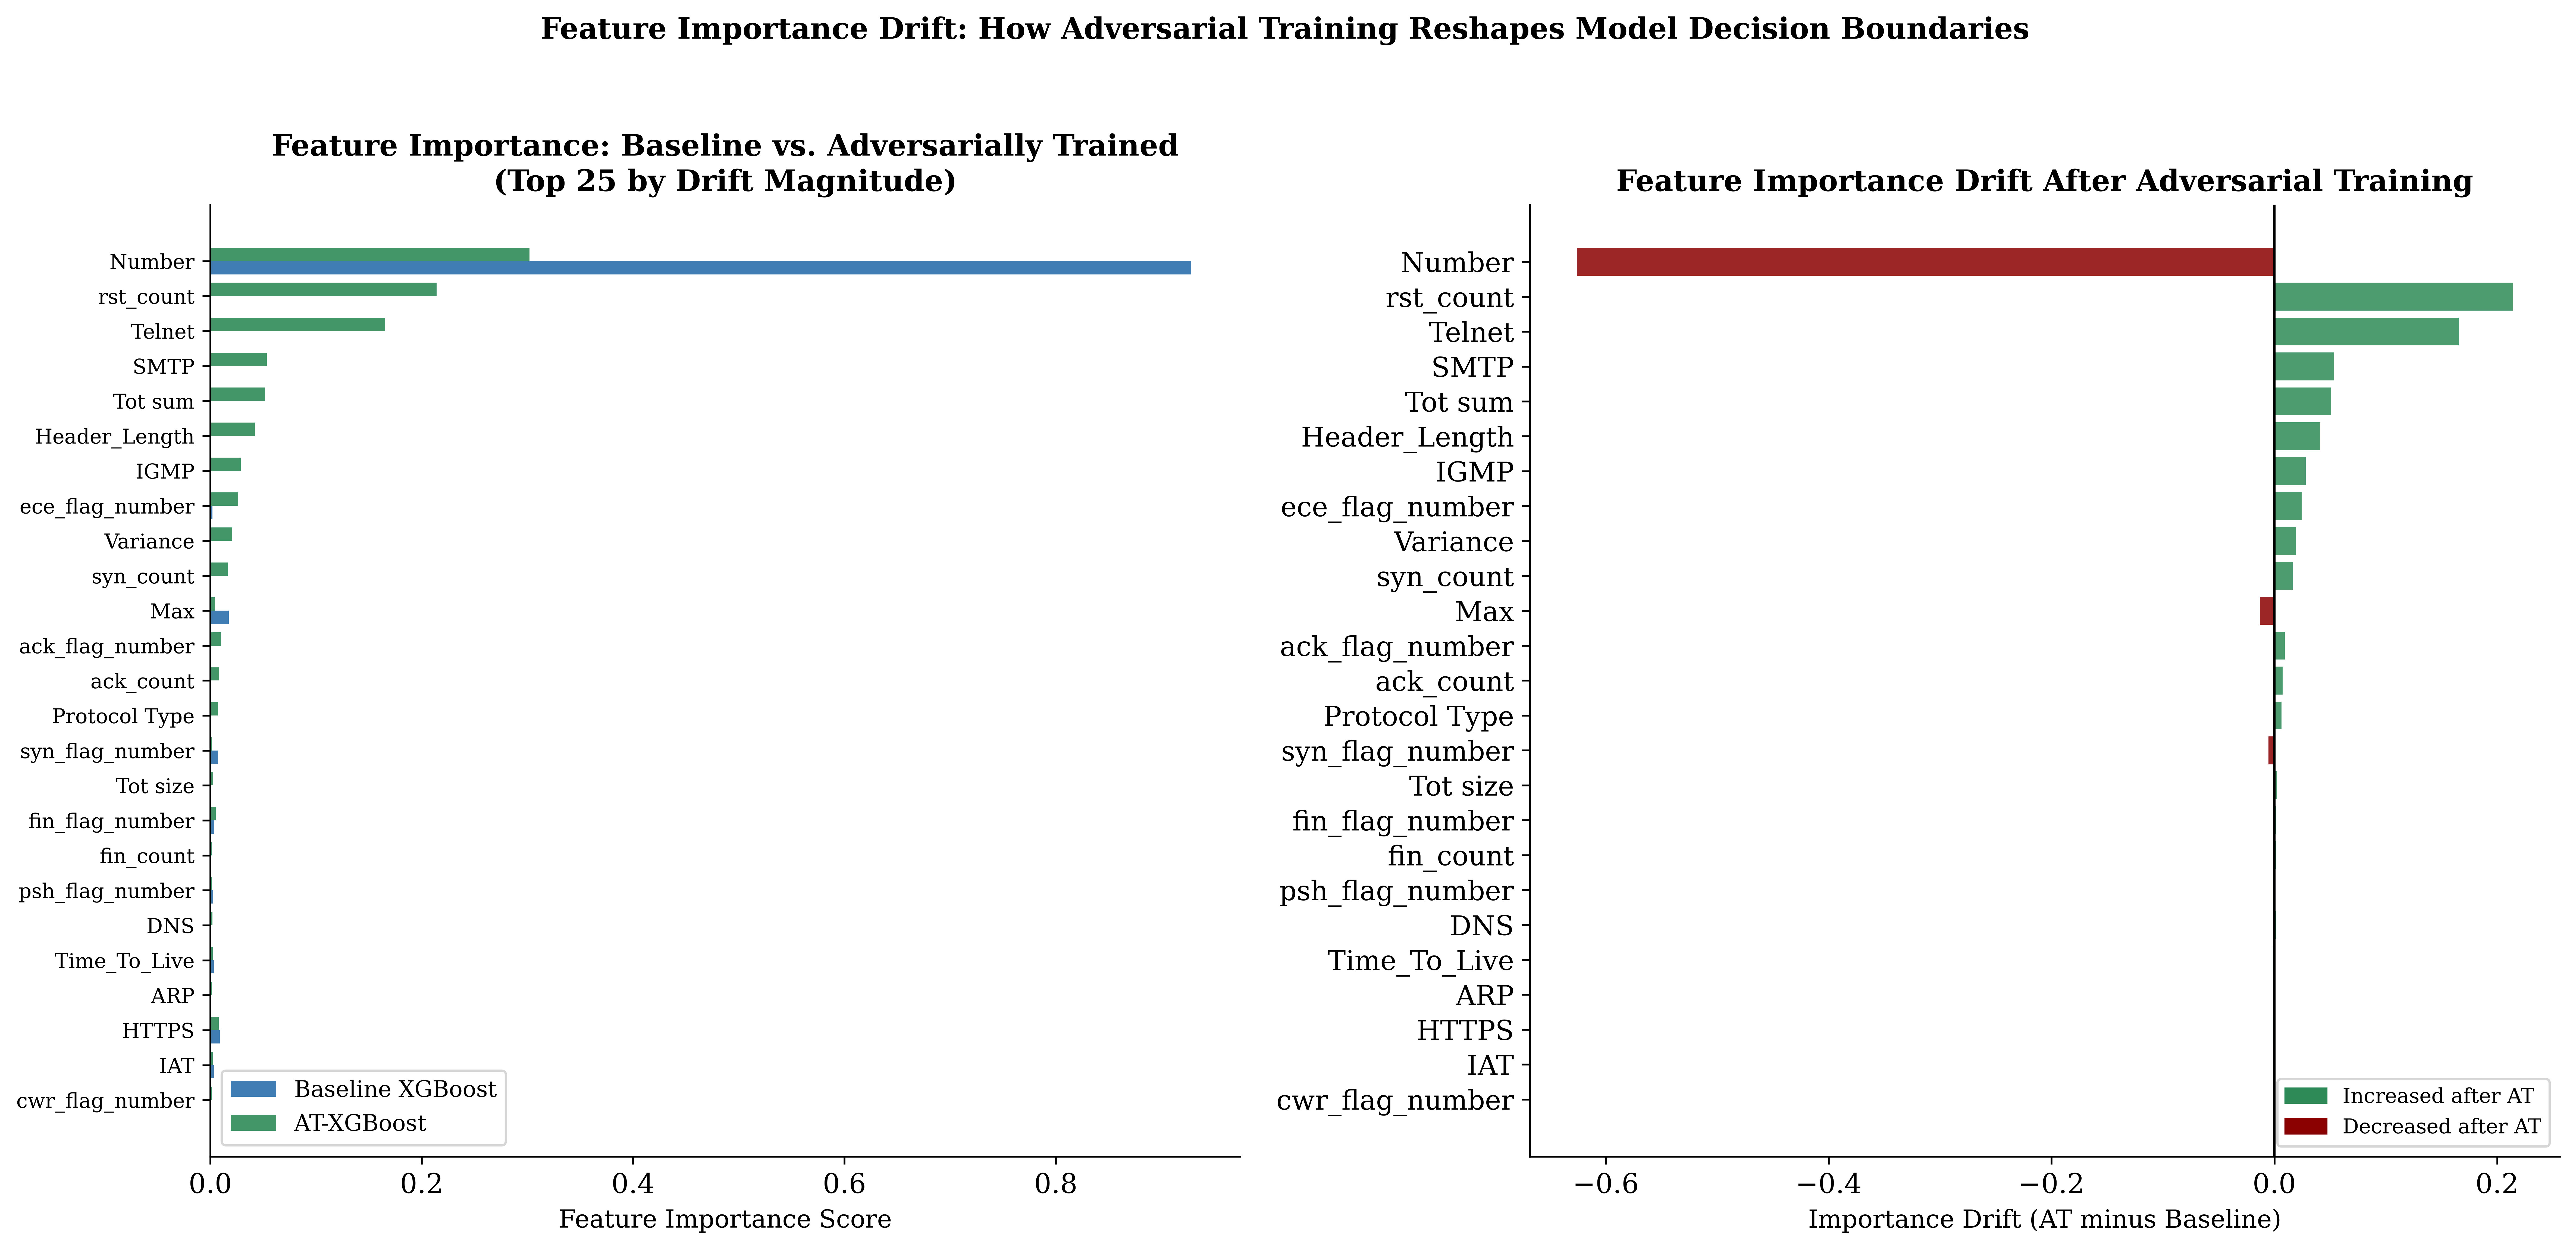
\includegraphics[width=0.9\textwidth]{../results/figures/fig21_feature_importance_drift.png}
% \caption{Feature importance drift after adversarial training.}
% \label{fig:drift}
% \end{figure}

\bibliography{references}

\end{document}
